\documentclass[conference]{IEEEtran} 
\IEEEoverridecommandlockouts

% 数式・単位・図表
\usepackage{amsmath,amssymb}
\usepackage{siunitx}
\usepackage{graphicx}
\usepackage{cite}
\usepackage[hidelinks]{hyperref}
\sisetup{detect-all=true}

% --- TikZ / PGF ---
\usepackage{tikz}
\usetikzlibrary{arrows.meta,positioning,shapes.geometric,shapes.misc,fit,calc}
\tikzset{
  mybox/.style = {rectangle, rounded corners, draw, fill=gray!12, minimum height=7mm, minimum width=24mm, align=center},
  mythin/.style = {line width=0.6pt},
  myarrow/.style = {-{Latex[length=2.2mm]}, line width=0.6pt},
  mynote/.style = {draw, fill=white, align=left, inner sep=2pt},
}

\title{Low-Cost Integration of 1.8-V FeFET on 0.18-\(\mu\)m CMOS:\\
+1 Mask and a Single ALD Tool, with Reliability Assessment}

\author{%
Shinichi Samizo\\
\emph{Independent Semiconductor Researcher}\\
Former Engineer at Seiko Epson Corporation\\
Email: \texttt{shin3t72@gmail.com}\\
GitHub: \url{https://github.com/Samizo-AITL}
}

\begin{document}
\maketitle

\begin{abstract}
This paper demonstrates the integration of a \SI{1.8}{V} FeFET module on a legacy \SI{0.18}{\micro m} CMOS process using only \textbf{one additional mask} and \textbf{a single ALD tool}. 
The fabricated devices show endurance exceeding \(10^{5}\) program/erase cycles and data retention longer than 10~years at \SI{85}{\celsius}. 
Time–zero and time–dependent dielectric breakdown (TZDB/TDDB), endurance, and retention were characterized on FeCAP/FeFET test structures. 
The proposed approach offers a cost-effective path to extend mature-node lifetimes and to enable embedded NVM for automotive/industrial/IoT.
\end{abstract}

\section{Introduction}
FeFETs based on HfO\(_2\) are promising CMOS-compatible embedded NVMs. 
While recent work targets advanced nodes, their adoption on mature nodes remains limited despite strong demand in automotive and industrial markets. 
Our contributions are: (i) \textbf{+1 mask} low-cost module, (ii) only \textbf{one ALD tool} added, (iii) yield-friendly SRAM+FeFET usage model, and (iv) comprehensive reliability evidence.

\section{Process Integration}
Baseline is a \SI{0.18}{\micro m} CMOS platform (\SI{1.8}{V} logic, optional \SI{3.3}{V} I/O). 
The FeFET module is inserted after poly definition and salicide/RTA. 
Stack: TiN / HZO (\SI{8}{–}\SI{12}{nm}, ALD) / Al\(_2\)O\(_3\) (\SI{1}{–}\SI{2}{nm}, ALD) / p-Si. 
Only one extra mask and one ALD tool are required; existing TiN sputter can be re-used.

\subsection{Process Flow}
\begin{figure}[t]
\centering
\begin{tikzpicture}[node distance=6mm]
\node (a) [mybox] {① FEOL 完了\\(Coシリサイド/RTA)};
\node (b) [mybox, below=of a] {② ダミーポリ除去};
\node (c) [mybox, below=of b] {③ ALD: Al$_2$O$_3$ (1--2 nm)};
\node (d) [mybox, below=of c] {④ ALD: HZO (8--12 nm)};
\node (e) [mybox, below=of d] {⑤ スパッタ: TiN (30--50 nm)};
\node (f) [mybox, below=of e] {⑥ RTA (450--500℃)};
\node (g) [mybox, below=of f] {⑦ BEOL 配線};

\foreach \u/\v in {a/b,b/c,c/d,d/e,e/f,f/g}{
  \draw[myarrow] (\u) -- (\v);
}
\end{tikzpicture}
\caption{FeFET プロセスフロー(0.18\,\textmu m CMOS)。}
\end{figure}

\subsection{Cross Section}
\begin{figure}[t]
\centering
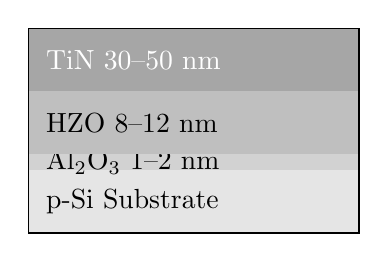
\begin{tikzpicture}[x=1mm,y=1mm]
\def\W{42}  
\def\Y{0}
\fill[gray!20] (0,\Y) rectangle (\W,\Y+8);
\node[anchor=west] at (1,\Y+4) {p-Si Substrate};
\fill[gray!35] (0,\Y+8) rectangle (\W,\Y+10);
\node[anchor=west] at (1,\Y+9) {Al$_2$O$_3$ 1--2 nm};
\fill[gray!50] (0,\Y+10) rectangle (\W,\Y+18);
\node[anchor=west] at (1,\Y+14) {HZO 8--12 nm};
\fill[gray!70] (0,\Y+18) rectangle (\W,\Y+26);
\node[anchor=west, text=white] at (1,\Y+22) {TiN 30--50 nm};
\draw[mythin] (0,\Y) rectangle (\W,\Y+26);
\end{tikzpicture}
\caption{HZO/Al$_2$O$_3$/TiN スタック断面模式図。}
\end{figure}

\section{Device and Methods}
Test structures include FeCAPs (flat/comb) and \SI{100}{\micro m}$\times$\SI{100}{\micro m} FeFET cells.
Programming conditions: $\pm2.3$–\SI{2.7}{V}, \SI{1}{–}\SI{50}{\micro s} pulses. 
Keysight B1500A and manual probing were used.

\section{Results}
\subsection{TZDB}
\includegraphics[width=\linewidth]{figures/fig3_tzdb.png}

\subsection{TDDB}
\includegraphics[width=\linewidth]{figures/fig4_tddb_cdf.png}
\includegraphics[width=\linewidth]{figures/fig4_tddb_weibull.png}

\subsection{Endurance}
\includegraphics[width=\linewidth]{figures/fig5_endurance.png}

\subsection{Retention}
\includegraphics[width=\linewidth]{figures/fig6_retention.png}

\section{System Architecture (SRAM + FeFET)}
\begin{figure}[t]
\centering
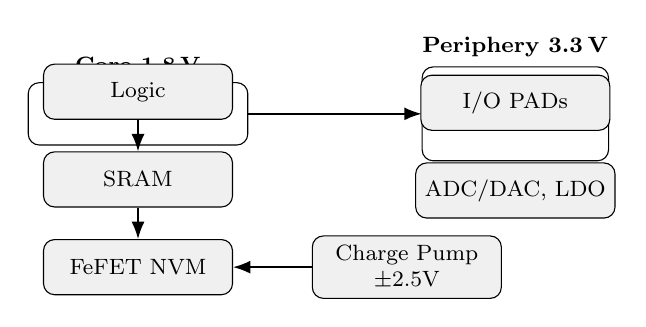
\begin{tikzpicture}[node distance=6mm, every node/.style={font=\footnotesize}]
\node[draw, rounded corners, inner sep=3mm, label=above:{\textbf{Core 1.8\,V}}] (core) {\phantom{MMMMMMMM}};
\node[draw, rounded corners, right=22mm of core, inner sep=5mm, label=above:{\textbf{Periphery 3.3\,V}}] (peri) {\phantom{MMMMM}};
\node[mybox, anchor=center] (logic) at ($(core.center)+(0,8pt)$) {Logic};
\node[mybox, below=4mm of logic] (sram) {SRAM};
\node[mybox, below=4mm of sram] (fefet) {FeFET NVM};
\node[mybox, right=10mm of fefet] (pump) {Charge Pump\\$\pm$2.5V};
\node[mybox, anchor=center] (io) at ($(peri.center)+(0,4pt)$) {I/O PADs};
\node[mybox, below=4mm of io] (ams) {ADC/DAC, LDO};
\draw[myarrow] (logic) -- (sram);
\draw[myarrow] (sram) -- (fefet);
\draw[myarrow] (pump) -- (fefet);
\draw[myarrow] (core.east) -- (peri.west);
\end{tikzpicture}
\caption{電源ドメイン構成。}
\end{figure}

\begin{figure}[t]
\centering
\begin{tikzpicture}[node distance=10mm]
\node[mybox] (s) {SRAM};
\node[mybox, right=16mm of s] (c) {Backup Ctrl};
\node[mybox, right=16mm of c] (f) {FeFET NVM};
\draw[myarrow] (s) -- node[above]{電断検知→Backup} (c);
\draw[myarrow] (c) -- (f);
\draw[myarrow] (f.south) |- ++(-12mm,-10mm) -| node[below]{復帰時リストア} (s.south);
\end{tikzpicture}
\caption{バックアップ/リストア経路。}
\end{figure}

\section{Discussion}
The HZO/Al$_2$O$_3$/TiN stack provides sufficient reliability for industrial/consumer embedded NVM. 
For high-temperature automotive, improvements are required: IL thickness optimization, crystallinity control, refresh operation, and ECC.

\section{Conclusion}
We realized an FeFET module on 0.18\,\textmu m CMOS with only \textbf{one extra mask} and \textbf{one ALD tool}. 
Devices exhibit $>10^5$ cycles and $>10$ years retention at \SI{85}{\celsius}. 
This extends mature-node lifetimes and enables cost-effective embedded NVM for automotive/industrial/IoT, though high-T retention remains limiting.

\section*{Acknowledgment}
The author thanks collaborators for helpful discussions.

\bibliographystyle{IEEEtran}
\begin{thebibliography}{99}
\bibitem{Boscke2011} T.~Böscke \emph{et al.}, \emph{Appl. Phys. Lett.}, vol.~99, p.~102903, 2011.
\bibitem{Mueller2012} J.~Müller \emph{et al.}, \emph{Appl. Phys. Lett.}, vol.~99, p.~112901, 2012.
\bibitem{Mikolajick2019} T.~Mikolajick \emph{et al.}, \emph{J. Appl. Phys.}, vol.~125, p.~204103, 2019.
\bibitem{Mueller2015} J.~Müller \emph{et al.}, \emph{IEEE TED}, vol.~62, no.~12, pp.~4158--4166, 2015.
\bibitem{Park2020} J.~Park \emph{et al.}, \emph{IEEE EDL}, vol.~41, no.~5, pp.~711--714, 2020.
\bibitem{Nakamura2003} H.~Nakamura \emph{et al.}, \emph{IEEE TDMR}, vol.~3, no.~4, pp.~132--136, 2003.
\bibitem{Yamazaki2018} K.~Yamazaki \emph{et al.}, \emph{Jpn. J. Appl. Phys.}, vol.~57, 04FB07, 2018.
\end{thebibliography}

\section*{Biography}
Shinichi Samizo has over 25 years of experience in semiconductor process integration and actuator development.  
After studying control theory and EM modeling in academia, he joined Seiko Epson in 1997 and worked on 0.35--0.18\,µm CMOS integration, DRAM, HV logic, and LCD drivers.  
Later he contributed to PZT actuator development and the PrecisionCore inkjet head.  
He is now an independent researcher, publishing open educational materials via the ``Project Design Hub''.
\end{document}
